\documentclass{article}
\usepackage{booktabs}
\usepackage{fancyhdr}
\pagestyle{empty}
\usepackage{graphicx}
 \usepackage{color}
 \usepackage{transparent}
 \usepackage{hyperref}
 \usepackage{lastpage}
 \usepackage[final]{pdfpages}
 
\pagestyle{fancy}
\lhead{} % Top left header
\chead{Heqet Tutorial} % Top center head
\rhead{} % Top right header
\lfoot{} % Bottom left footer
\cfoot{} % Bottom center footer
\rfoot{ \thepage/\protect\pageref{LastPage}} % Bottom right footer \protect\pageref{LastPage}

\newcommand{\prob}[1]{\noindent\textbf{#1.}}

\begin{document}
\pagestyle{empty}
\begin{center}
\vspace{3cm}
\scalebox{1.5}{{\Huge Heqet Tutorial}}

\vspace{2cm}
{\Large By Isaac Reilly}

\vspace{0.15cm}
{\large advised by Donya Quick}

\vspace{0.1cm}
{senior project for the Yale University major in Computer Science}

\vspace{13cm}

{\small fall 2015}

\end{center}

\pagebreak

\tableofcontents
\newpage
\pagestyle{plain}

\begin{section}{Heqet for Euterpea Users}
Given a Euterpea music expression, creating a score is
 straightforward. You will need to import \verb+Heqet+ 
 and \verb+Heqet.Input.Euterpea+ and then apply the following functions:
First, to convert it to a Heqet music value, 
you should use \verb+fromEu+ or \verb+fromEu1+, which take a Euterpea \verb+Music Pitch+ or a \verb+Music Note1+ respectively. Now you can print a score to
 stdout with the functions \verb+quickScore+ or \verb+quickLine+. \verb+quickScore+ produces a piano rendition, while \verb+quickLine+ writes a single staff. 
 
 The reason that these functions perform IO is that the 
 simplest way to use Heqet is to write a Haskell program which outputs your Lilypond code and 
 pipe it directly into Lilypond, which you can do by running the included \verb+heqet.sh+ bash script with your Haskell program filename as an argument. Alternatively, just load your program into GHCi and paste the output code into a Lilypond file.

Now, let's try something more complicated. Suppose you have a score that has multiple instruments and you want to write them on separate staves with appropriate labels. If your Euterpea music value has instrument modifiers, you can just use \verb+writeScore+ for your output function, since Euterpea instruments are converted automatically. If you don't have instrument modifiers, or if your instruments are beyond the basic set of instruments currently recognized, you'll have to assign instruments in Heqet. The tools to manipulate music are mostly lenses, best used with the \verb+Control.Lens+ package. Lenses and other ``optics'' are a way to modify portions of a larger piece of data, for example, changing the instrument assigned to some of the notes of a music value. 

By the way, this is a good time to mention that in Heqet most properties of music are recorded on every single note they impact. So, every note has a field for its \verb+Maybe Instrument+. This way, you can rearrange the music as much as you want without worrying about handling the transitions between states over the course of the music---if the instrument changes, then Heqet is supposed to automatically write this direction into the part.(Actually, this isn't implemented yet. An example that does work is handling slurs: a slurred is considered to be an articulation on all but the last note in the slur. If you cut a slurred phrase in half, both halves will stay slurred correctly.) 

Suppose we have a Heqet music value \verb+opus+. Let's make it played by an oboe:

\verb+opusWithInstruments = opus & traverse.val.inst .~ Just oboe+

Quick explanation of these operators: \verb+traverse.val.inst .~ Just oboe+ is a function that can manipulate some music. \verb+&+ is a \verb+flip+ed  \verb+$+. So we're applying this function to \verb+opus+. In the middle is the ``optic'', or in this case a composition of three: \verb+traverse+, \verb+val+, and \verb+inst+. \verb+traverse+ looks at every note in the music, \verb+inst+ looks at the instrument of a note, and \verb+val+ is an implementation detail that will be hidden in future versions of Heqet. The \verb+.~+ operator means to set the value revealed by the optic, in this case setting the instrument field of every note to be \verb+Just oboe+. 

Suppose that all but one instrument was recognized automatically. Then, we could set all the notes with an unknown instrument to be an oboe like this:

\begin{verbatim}opusWithInstruments = opus 
    & instKind "Unknown".traverse.val.inst .~ Just oboe
\end{verbatim}

\verb+instKind+ is a function that takes a string and produces a lens that looks at notes which have
an instrument of that kind. The unknown instrument is a real instrument, not just a value of \verb+Nothing+ in the instrument field, because we need to know how to write its name in a score, what clefs it uses, what range it has (unlimited), etc. 

If you try these examples, you might notice a problem: all the music is still on one staff! That's because staff assignments are separate from instrument assignments. To assign a staff of \verb+"3"+ (yes, that's a string) to the Bari Sax, we write:

\begin{verbatim}opusWithInstruments = opus 
    & instKind "Bari Sax".traverse.val.line .~ Just "3"
\end{verbatim}

Heqet provides lenses to select music by start and end time or by any predicate on a single note. 

To output a score with correct note durations, you need to assign a meter.  The meter is one of the rare musical properties that is not stored in the notes themselves. Rather, a meter is a set of notes which, instead of having pitches, have measure and beat events. Assigning a meter to a segment of music simply means inserting these notes, which can have a staff just like any other note. These events can be sliced and moved around with their music, and  Heqet will analyze them to determine what meter they specify and where meter changes need to be inserted into the printed score. To make a piece of music in common time, write:

\begin{verbatim}opusWithInstruments = opus 
    & assignMeter m4_4
\end{verbatim}

Even though \verb+assignMeter m4_4+ does not use a lens, I find it natural to apply it with \verb+&+, since often I want to take a music value and apply many functions to it, writing each function on a separate line beginning with the \verb+&+. 

(note: meter rendering has developed a bug which I don't have time to fix as I have stopped coding to write up my report and tutorial. Meters now simply don't appear in the rendered code.)

If you want the string output by \verb+writeScore+, you can use \verb+allRendering+ instead, but I don't expect this to be a common need.

\end{section}

\begin{section}{Heqet for Lilypond Users}
So you want to do some fancy computer processing of your music, but you're not hot about Scheme, or at least are frustrated with the limited tools for working with Lilypond music data? You've come to the right place! However, this tutorial will not teach Haskell. 

\begin{subsection}{Note input}
In order to enter music into Haskell source code using the Heqet DSL, you need to enable the  ``quasi-quoting'' optional language feature by either putting \verb+{-# LANGUAGE QuasiQuotes #-}+ at the top of your source file or by typing \verb+:set -XQuasiQuotes+ into GHCi. Then import Dutch or English note entry with 

\verb+import Heqet.Input.Dutch+

\verb+import Heqet.Input.English+

Now you can create Heqet music values in Haskell by writing them enclosed by ``\verb+[music|+'' and ``\verb+|]+'', like so: 

\verb+[music| c4 d8 e f2 |]+

\end{subsection}

\begin{subsection}{Differences from Lilypond input}
There are several differences between the Heqet note-input domain-specific language and Lilypond input, for a variety of reasons, including philosophical differences, features Heqet provides which are not in Lilypond, features which would be troublesome to implement in Heqet, and features which I simply haven't gotten around to yet. 
\begin{itemize}
\item You can enter notes with any rational duration with the \verb+\d+ syntax, for example \verb+c\d 4/5+ to make a note with a duration of $4/5$ of a whole note. You can omit the denominator if it's $1$. This is currently the only way to enter notes of the durations needed for a tuplet.

\item You can also enter notes with any frequency you like by writing the pitch as a number followed by  \verb+hz+, for instance \verb+[music| 234.01hz4. |]+

\item You can modify the pitch of a note with the command \verb+\cents+ followed by a number, possibly negative. This is currently the only way to get a quarter-tone pitch.

\item The only languages you can currently use are Dutch and English. 

\item At the moment, slurs must be entered by putting a \verb+-(+ articulation on every note but the last.

\item You cannot enter clefs, keys, or time signatures. I might implement time signatures, but Heqet will never support keys or clefs in note entry, since these are matters of how music is presented to the musician, not fundamental aspects of the music itself.

\item Lilypond is actually difficult to parse because there is no syntactic difference between a command like \verb+\fermata+, which follows the note it applies to, and one like \verb+\xNote+, which proceeds its argument. In addition, many Lilypond commands change the state of all music that follows it, but not all do. Given the obvious usefulness of importing directly from Lilypond, in the future I will probably write some sort of Scheme tool to run in Lilypond and create a Heqet music value. 

This means that if you want to include Lilypond commands, you must specify their syntax. If a command follows its note, begins with a backslash, and contains only alphanumeric characters, then you can write it as in Lilypond. If it follows its note but doesn't meet these criteria, enter it with \verb+\with+ and your desired command in a string: \verb+c4 \with "\\foo 1.7"+. If you have a command that has a part that proceeds its music argument, for instance the pair of \verb+\stopStaff+ and \verb+\startStaff+ to temporarily hide the staff, then you must enter it as follows:

\begin{verbatim}
[music| c4 \command "\\stopStaff" "\\startStaff" { c d } e |]
\end{verbatim}

Since many Lilypond commands take their music argument in braces, with the closing brace being the only part that follows the music, there is a shortcut:

\begin{verbatim}
[music| c4 \function "\\transpose c e" { c d } e |]
\end{verbatim}

A Lilypond command is separately recorded on every note it's applied to. At the moment, no effort is made to combine notes with a certain command into a single instance of that command with a long music argument upon rendering. This will be required for rendering octava marks correctly, and may improve performance, so future versions of Heqet may include a way to mark whether a command must, can, or shouldn't be combined.

A warning: although it is possible to insert arbitrary Lilypond code into a Heqet music value, please take care, as rearranging the notes of a heavily-tweaked piece of music might have unexpected effects, as Heqet currently has no understanding of the meanings of Lilypond commands.

\item Currently, only absolute note entry is possible. 

\item In Lilypond, you can enter regular notes or you can enter percussion notes in drum mode. In Heqet, both kinds of notes are mixed. You must enter percussion notes by proceeding each with \verb+\p+, so \verb+\phh+ means a hi-hat note. 

\item There is no way to manually specify beams, and never will be.

\item Repeats are not supported in note entry and probably never will be, as they are matters of notation, not musical fundamentals, and it's easy to repeat a section of music using Haskell functions without resorting to notation in the music-entry DSL.

\end{itemize}
\end{subsection}
\end{section}

\begin{section}{More processing}
To combine pieces of music in parallel or in sequence, use the functions \verb+parI+ and \verb+seqI+. A piece of music in Heqet exists at a specific time. \verb+seqI+ will move its second argument to immediately follow its first, while \verb+parI+ simply squashes the two segments of music together into one no matter what time they occur. To change the time that a piece of music starts at, use the function \verb+startMusicAt+, which takes a rational starting time and a piece of music. For example, \verb+seqI+ is defined as

\begin{verbatim}
seqI m1 m2 = m1 `parI` (startMusicAt (getEndTime m1) m2)
\end{verbatim}

where \verb+getEndTime+ and its companion \verb+getStartTime+ do the obvious. If you want to modify a section of music specified by its start or end time, you can use the functions \verb+takeMusic+, \verb+dropMusic+, and \verb+sliceMusic+, which take 1 or 2 rational points in time and give a lens which can be used to focus on that section of music. To discard the other parts of the music, you can ``view'' the music through the lens with the \verb+^.+ operator, for instance \verb+opus ^. sliceMusic 0 100+
\end{section}


\begin{section}{Making your own note type}
Say you want to play around with 19-tone equal temperament. Heqet currently doesn't have built-in support for notes other than 12-tone equally tempered pitches, percussion, and lyrics, but you can still create your own type of pitch, put it in a \verb+Music+ value (even mixed with other types of pitches) and render it to Lilypond. You'll need to turn on the DeriveDataTypeable extension by putting 
\verb+{-# LANGUAGE DeriveDataTypeable #-}+ in your source file or typing \verb+:set -XDeriveDataTypeable+ in GHCi. Now, \verb+import Data.Typeable+. Then define your new pitch type, deriving \verb+Show+ and \verb+Typeable+. Now, Heqet defines a data contractor called \verb+Ly+ which can take any argument that implements \verb+Show+ and \verb+Typeable+, as well as two Heqet classes, \verb+Renderable+ and \verb+Playable+. Now look at \verb+LyInstances.hs+ and the beginning of \verb+Output/Render.hs+ for example instances and write your own.

\begin{verbatim}
class Renderable a where
    renderInStaff :: (Note MultiPitchLy) -> a -> String
    getMarkup :: a -> [String]
    isDisruptive :: a -> Bool

class Playable a where
    info :: a -> Maybe PlayInfo

data PlayInfo = PlayInfo {
    _slurrable :: Bool
  , _chordable :: Bool
  , _pitchHeight :: Maybe Double
    }
\end{verbatim}

\end{section}
\begin{section}{Example}
\begin{verbatim}
polyPiano = [music| 
<< { c1 } \\ 
{c''8. c''16 d''4 e'' f''} \\ 
{ r4 r8 g''8 bf''8 r8 r4 } >> 
c8 e g c' e' g' c'' e'' <c''' c''>1 |]
    & assignMeter m4_4
    & superBasicSplit
    & traverse.val.inst .~ Just Instruments.piano
\end{verbatim}
This example demonstrates chords, polyphony, and automatic splitting of music into two staves for piano.

\begin{figure}
 \centering 
 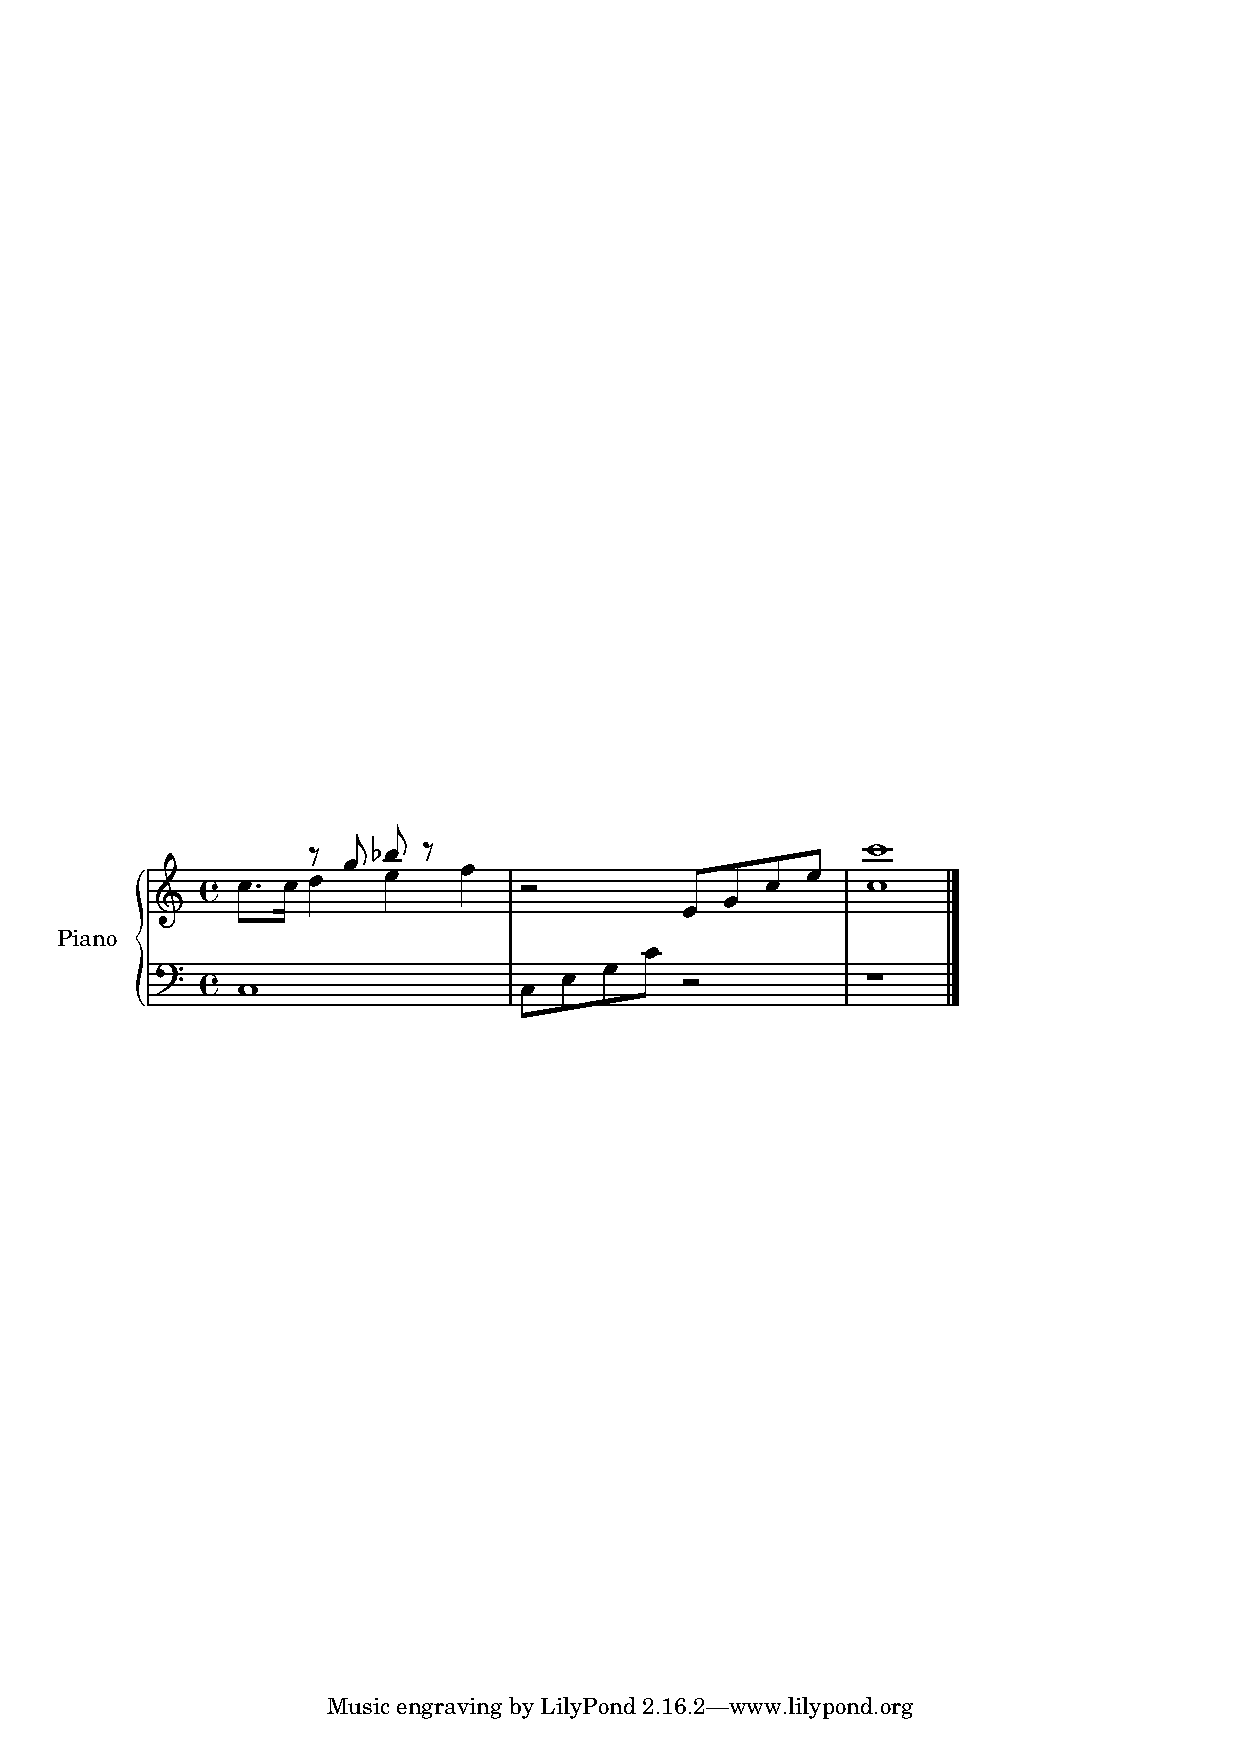
\includepdf[pages=-]{polyPiano.pdf}
\end{figure}

More examples are in \verb+TestCases.hs+.

\end{section}
\end{document}